\begin{exercise}
\begin{figure}[H]
\centering
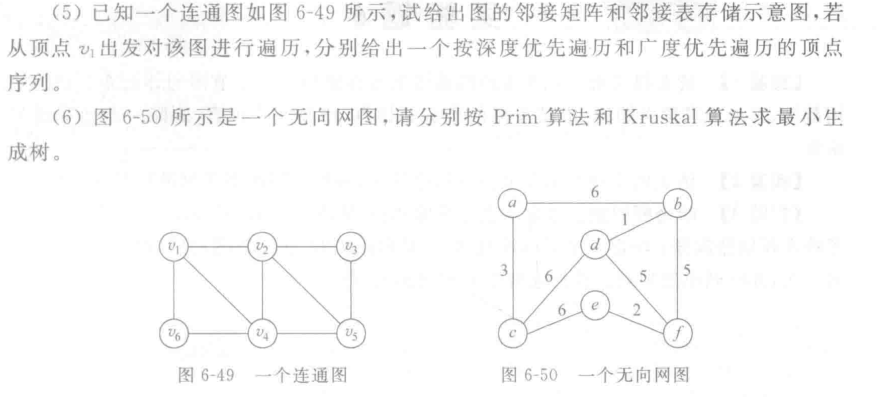
\includegraphics[width=\textwidth]{1-hw7-2025061022.png}
% \caption{}
\label{}
\end{figure}
\end{exercise}
\begin{figure}[H]
\centering
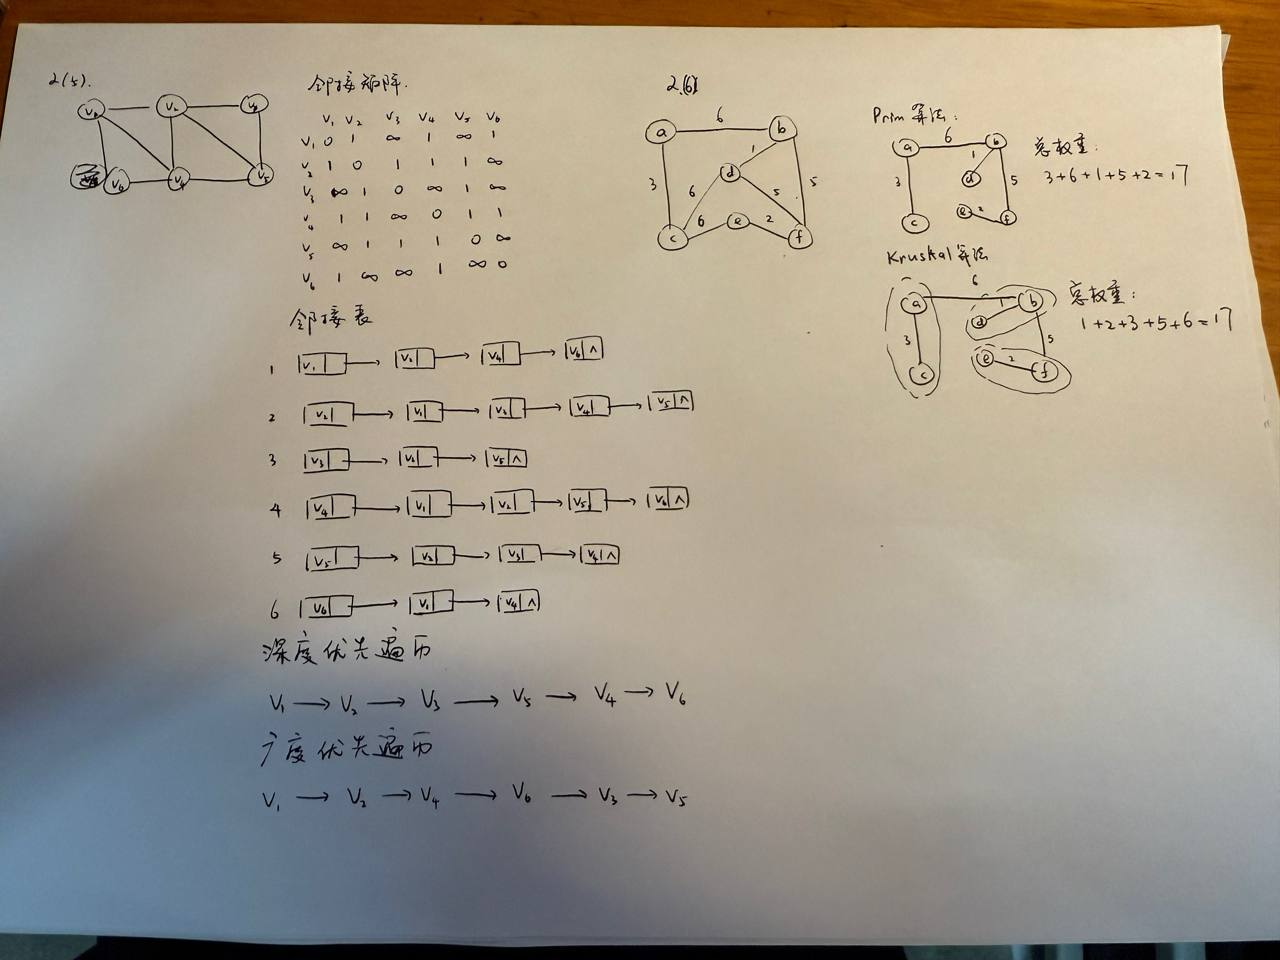
\includegraphics[width=\textwidth]{hw7-2025061022.png}
% \caption{}
\label{}
\end{figure}

\begin{exercise}
\begin{figure}[H]
\centering
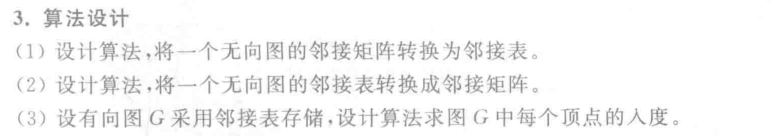
\includegraphics[width=\textwidth]{2-hw7-2025061022.png}
% \caption{}
\label{}
\end{figure}
\end{exercise}
(1)

\begin{lstlisting}
输入:n x n 的邻接矩阵 M, 顶点数 n
输出:邻接表 Adj

1. 遍历 n 个顶点,对于顶点 i,考虑它与这 n 个顶点的连接情况,从第 1 个开始数,若与第 j 个顶点相连,即 M[i][j] == 1,那就把这个顶点指向 j,即 Adj[i].next = j.
2. 以此类推,若与下一个顶点 k 相连,则 Adj[i].next.next = k,直到 j 遍历完这 n 个顶点,i 遍历完这 n 个顶点.

\end{lstlisting}
(2)

\begin{lstlisting}
输入:邻接表 Adj, 顶点数 n
输出:n x n 的邻接矩阵 M

1. 遍历 n 个顶点,对于顶点 i,令 p = Adj[i],那么赋值 M[i][p.adjvex] = 1,再令 p = p.next,以此类推,直到 p == NULL.
2. 赋值 M[i][i] =0,其他空的位置赋值为无穷大♾️
\end{lstlisting}
(3)

\begin{lstlisting}
输入:邻接表 Adj, 顶点数 n
输出:n 个顶点的入度 indeg

1. 遍历 n 个顶点,对于顶点 i,先赋值 indeg[i] = 0.
2. 然后遍历 n 个顶点,对于顶点 j,令 p = Adj[j].next,若 p.adjvex == i,则 indeg[i] = indeg[i] + 1. 令 p = p.next,以此类推,直到 p == NULL.
3. 最后得到对于每个 i 的 indeg[i] 值.

\end{lstlisting}